\begin{frame}
\frametitle{A symmetric electron-positron theory (1937)}
\begin{columns}
\column{0.35\textwidth}
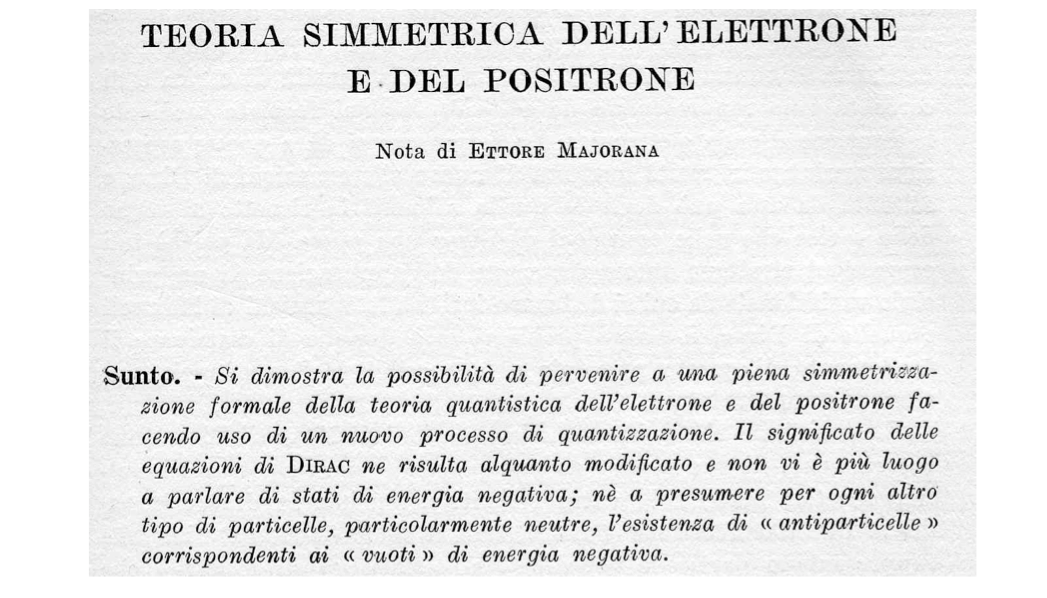
\includegraphics[scale=0.32]{img/MajoranaPaper.png}
\column{0.35\textwidth}
We show that it is possible to achieve complete formal symmetrization in the electron and positron quantum theory by means of a new quantization process. The meaning of Dirac equations is somewhat modified and {\bf it is no more necessary to speak of negative-energy states; nor to assume, for any other type of particles, especially neutral ones, the existence of antiparticles, corresponding to the ``holes'' of negative energy.}
\end{columns}
\end{frame}

%\begin{frame}
%\frametitle{An unpleasant symmetry}
%\begin{itemize}
%\item ``The interpretation of the so called ``negative energy states'' proposed by Dirac leads, as it is well known, to a substantially symmetric description of electron and positrons... but it looks to us important, in view of possible extensions, that the notion itself of negative energy state be abandoned." 
%\item ``Indeed, we shall see that to be perfectly possible to build, in the most natural way, a theory of the neutral elementary particles without negative states."
%\item ``The new approach allows not only to give a symmetric form to the electron-positron theory, but also to build a substantially novel theory for the particles deprived of electric charge."
%\item ``it is probably not yet possible to ask to the experience to decide between this new theory and the simple extension of the Dirac equations to the neutral particles."
%\end{itemize}
% 
% \alert{VOW!}
% 
%\begin{itemize}
%\item At the time the neutrino had not yet been discovered. 
%\item Even if in those times the only known ``charge'' was the electric charge, Majorana implicitly assumed particles deprived of \alert{all the possible charges}. 
%%\item Eighty years later we have not yet been able to decide between Dirac and Majorana theories.
%%\item But we hope we will be able to tell in maybe another ten or twenty years.
%\end{itemize}
%\end{frame}

\begin{frame}
\frametitle{Majorana's approach}
Majorana questioned whether it was necessary for spin-1/2 particles to have equations that involved complex numbers. What was required were gamma matrices that still satisfy the Clifford algebra but were purely imaginary. Majorana found such constructions in terms of the Pauli matrices:
\[
\gamma^0 = \mqty(0 & \sigma_2 \\ \sigma_2 & 0), \,\,\,
\gamma^1 = \mqty(i \sigma_1 & 0 \\ 0 & i \sigma_1), \,\,\,
\gamma^2 = \mqty(0 & -\sigma_2 \\ \sigma_2 & 0), \,\,\,
\gamma^4 = \mqty(i \sigma_3 & 0 \\ 0 & i \sigma_3)
\]
Recall that $\sigma_1, \sigma_3$~are real, while $\sigma_2$~is complex. Thus, all the Majorana gamma matrices are complex. But then, the Majorana spinor $\psi_M$~must be real \alert{and is therefore invariant to charge conjugation}. The derived field theory can be constructed from one type of operator. Therefore, the particles created \alert{are fermions that are their own antiparticles}.
\end{frame}
%
%\begin{frame}
%\frametitle{Dirac revisited}
%In modern QED we interpret the solutions of the Dirac equation as a 4-dimensional spinor $\psi$~is a:
%\[
%\psi = \mqty(\psi_1 \\ \psi_2 \\ \psi_2 \\ \psi_4) = \mqty(\phi \\ \chi)
%\]
%where $\phi =  \mqty(\phi_1 \\ \phi_2)$ represents a particle (with two spin states) and
%$\chi =  \mqty(\chi_1 \\ \chi_2)$ represents an antiparticle (also with two spin states).
%\end{frame}
%
%\begin{frame}
%\frametitle{Dirac equation using Weyl representation of the $\gamma$~matrices}
%\[
%\gamma^0  = \mqty(0 & I \\ I & 0),\,\,\, \gamma^i  = \mqty(0 & -\sigma^i \\ \sigma^i  & 0)
%\]
%Then the Dirac equation becomes:
%\[
%\left[ E  \mqty(0 & I \\ I & 0) - \mqty(0 & -\va{p}\cdot\va{\sigma} \\ \va{p}\cdot\va{\sigma}  & 0) -m \right]
% \mqty(\phi \\ \chi) = 0
%\]
%which solves into two equations:
% \begin{empheq}[box=\fbox]{align}
%(E +  \va{p}\cdot\va{\sigma}) \chi - m \phi & = 0 \nonumber \\
%(E -  \va{p}\cdot\va{\sigma}) \phi - m \chi & = 0 \nonumber
%\end{empheq}
%
%The first equation represents particles (electrons) while the second represent antiparticles (positrons). In each equation, the helicity states (left-handed and right handed) are coupled through the particle mass. Notice that we can "assign" unambiguously two solutions two {\it matter} ($e^-$) and two solutions to {\it antimatter} ($e^+$), given the fact, dictated by nature that positrons and electrons are electrically charged particles (with opposite charges). 
%\end{frame}
%
%\begin{frame}
%\frametitle{Electron mass in modern QFT: coupling helicity states to the Higgs Field}
%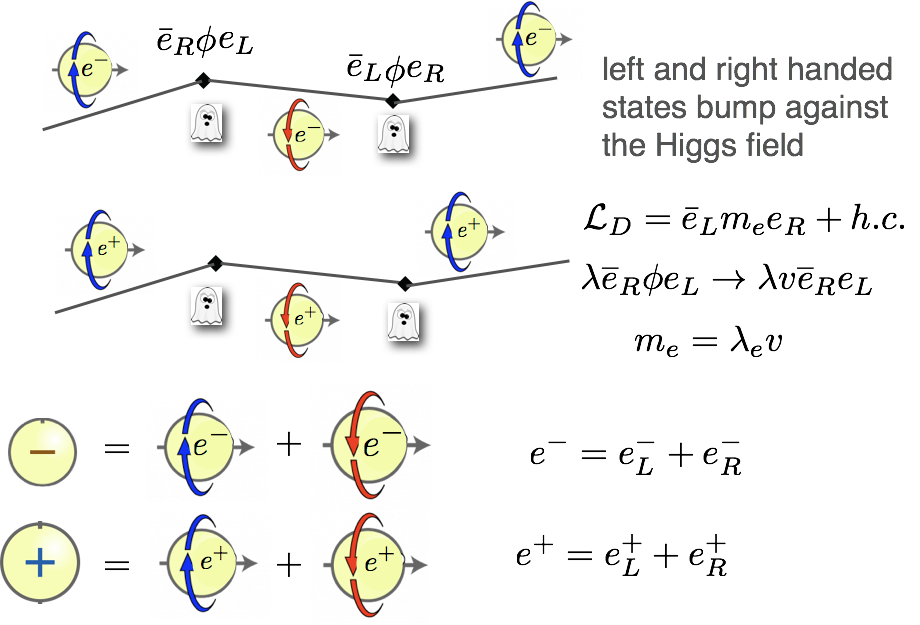
\includegraphics[scale=0.30]{img/ElectronMass.png}
%\end{frame}
%
%
%\begin{frame}
%\frametitle{Massless particles}
%In the limit of $m \rightarrow 0$~ these two equations decouple and we obtain
%two states with definite helicity:
% \begin{empheq}[box=\fbox]{align}
%(E +  \va{p}\cdot\va{\sigma}) \chi  & = 0 \nonumber \\
%(E -  \va{p}\cdot\va{\sigma}) \phi  & = 0 \nonumber
%\end{empheq}
%Notice that we have now only two degrees of freedom, since the particle has negative helicity and the antiparticle positive helicity. 
%
%\end{frame}
%
%
\begin{frame}
\frametitle{Majorana insight}
Majorana proposed an alternative to the two-coupled, two-component Dirac equation, namely two independent, relativistic, two-component equations:

 \begin{empheq}[box=\fbox]{align}
(E +  \va{p}\cdot\va{\sigma}) \chi - m \epsilon \chi^* & = 0 \nonumber \\
(E -  \va{p}\cdot\va{\sigma}) \phi - m \epsilon \phi^* & = 0 \nonumber
\end{empheq}
where
\[
\epsilon = i \sigma_2 = \mqty(0 & I \\ -I & 0)
\]
If we compare with the Dirac equation:
 \begin{empheq}[box=\fbox]{align}
(E +  \va{p}\cdot\va{\sigma}) \chi - m \phi & = 0 \nonumber \\
(E -  \va{p}\cdot\va{\sigma}) \phi - m \chi & = 0 \nonumber
\end{empheq}
It's obvious that both equations are identical for $m=0$. In the Standard Model neutrinos are assumed to be massless and thus both theories are identical. Instead, if neutrinos are massive they are not. The remarkable thing about Majorana equation is that it is constructed only with the $\phi$ (or the $\chi$ for the second equation), thus eliminating two degrees of freedom. 
\end{frame}

%\begin{frame}
%\frametitle{Is the neutrino its own antiparticle?}
%\alert{A particle is its own antiparticle if we can reverse all its charges without effect}. Obviously electrons cannot be their own antiparticles, but Dirac neutrinos are also not their own antiparticles, as explicit in the construction of the bi-spinor that separates particles ($\phi$) and antiparticles ($\chi$).
%
%Given a spinor $\phi$~representing a particle, the charge-conjugate spinor representing an antiparticle is:
%
% \begin{empheq}[box=\fbox]{align}
% \phi^C & = C \gamma^0 \phi^*\nonumber
%\end{empheq}
%%\[
%%\phi^C = C \gamma^0 \phi^* 
%%\]
%where $\phi^*$~is the complex conjugate of $\phi$ and the charge conjugation matrix $C$~can be written in the Weyl representation as:
%\[
%C = \mqty(-i\sigma_2 & 0 \\ 0 & i\sigma_2), \,\,\, C \gamma^0 = \mqty(0 & -i\sigma_2 \\ i \sigma_2 & 0)
%\] 
%\end{frame}
%
%\begin{frame}
%For a Majorana spinor $\phi  \mqty(\phi \\ i \sigma_2 \phi^*)$:
%\begin{empheq}[box=\fbox]{align}
%\phi^C & = C \gamma^0 \phi^* =  \mqty(0 & -i\sigma_2 \\ i \sigma_2 & 0) \mqty(\phi^* \\ -i \sigma_2 \phi) \\
%& =\mqty(-i^2 \sigma^2 \phi \\ i \sigma_2 \phi^*) = \mqty(\phi \\ i \sigma_2 \phi^*) = \phi
%\nonumber
%\end{empheq}
%Thus, \alert{a Majorana particle is identical to its antiparticle.}
%\end{frame}
%
%\begin{frame}
%\frametitle{Majorana neutrinos violate lepton number}
%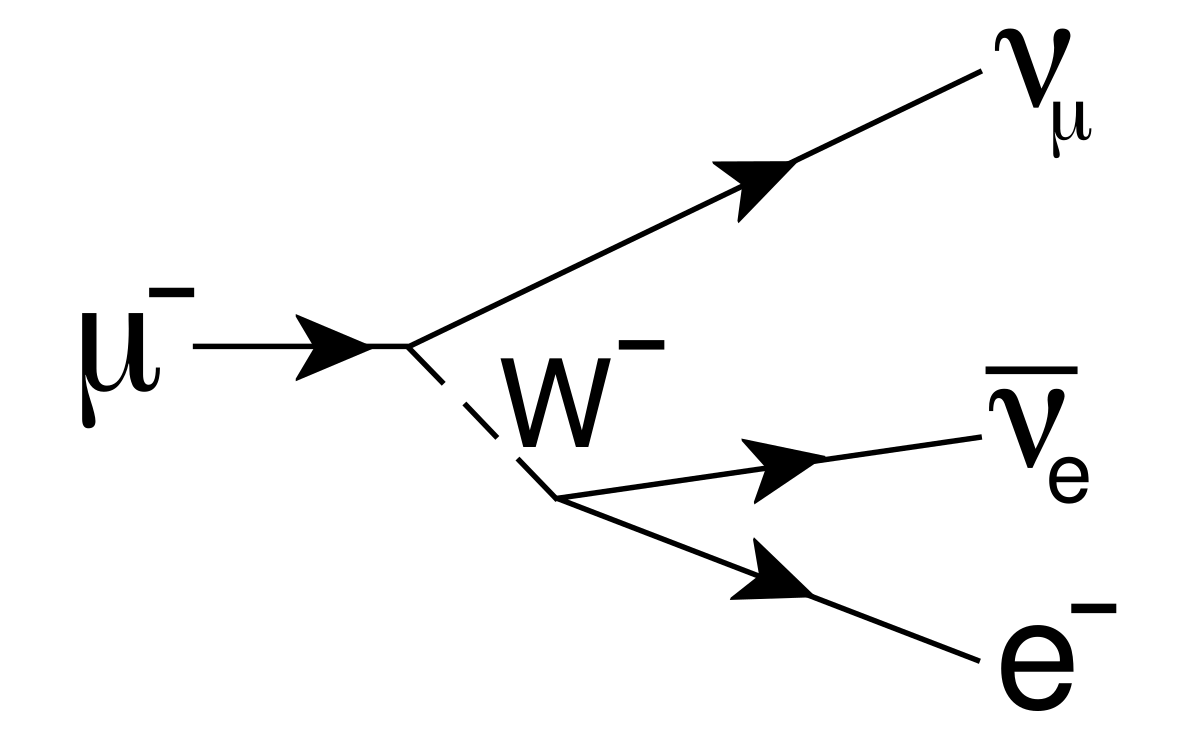
\includegraphics[scale=0.08]{muonDecay.png}
%
%Lepton number counts the total number of leptons and anti-leptons involved in a weak interaction which must be zero. For example, in the
%decay of $\mu$~above, the disappearance of the $\mu^-$~ (a lepton) is compensated with the appearance of a $\nu_\mu$~(also a lepton), while the appearance of $e^-$~(a lepton) is compensated with the
%appearance of a $\bar{\nu_e}$~(an anti-lepton). On the contrary, Majorana neutrinos have no lepton number. As such they may induce processes violating lepton number conservation.
%
%In most processes involving neutrinos the energy of the process is very large compared with the (tiny) neutrino mass. In practice we approach the limit $m=0$~and Dirac and Majorana become impossible to distinguish. 
%
%\end{frame}
%

\begin{frame}
\frametitle{Majorana neutrinos}
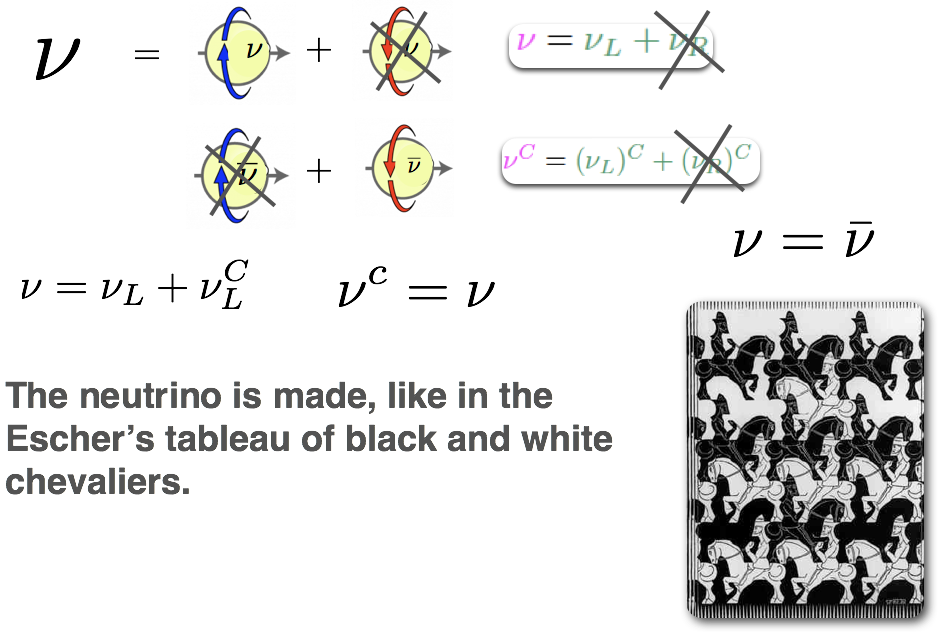
\includegraphics[scale=0.30]{img/MajoranaNeutrinosCartoon.png}
\end{frame}

%\begin{frame}
%\frametitle{Majorana mass}
%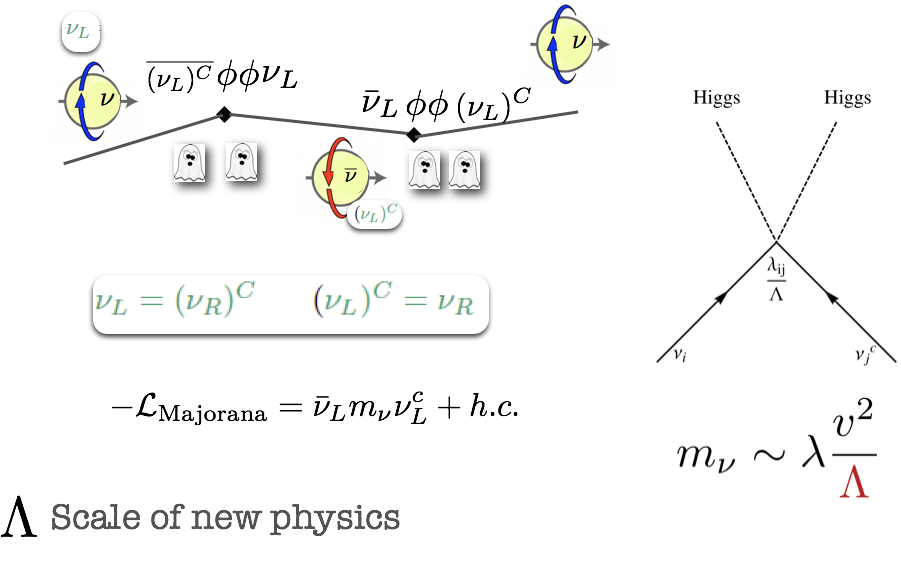
\includegraphics[scale=0.30]{img/MajoranaMass.png}
%\end{frame}

%\begin{frame}
%\frametitle{Majorana and Dirac neutrinos}
%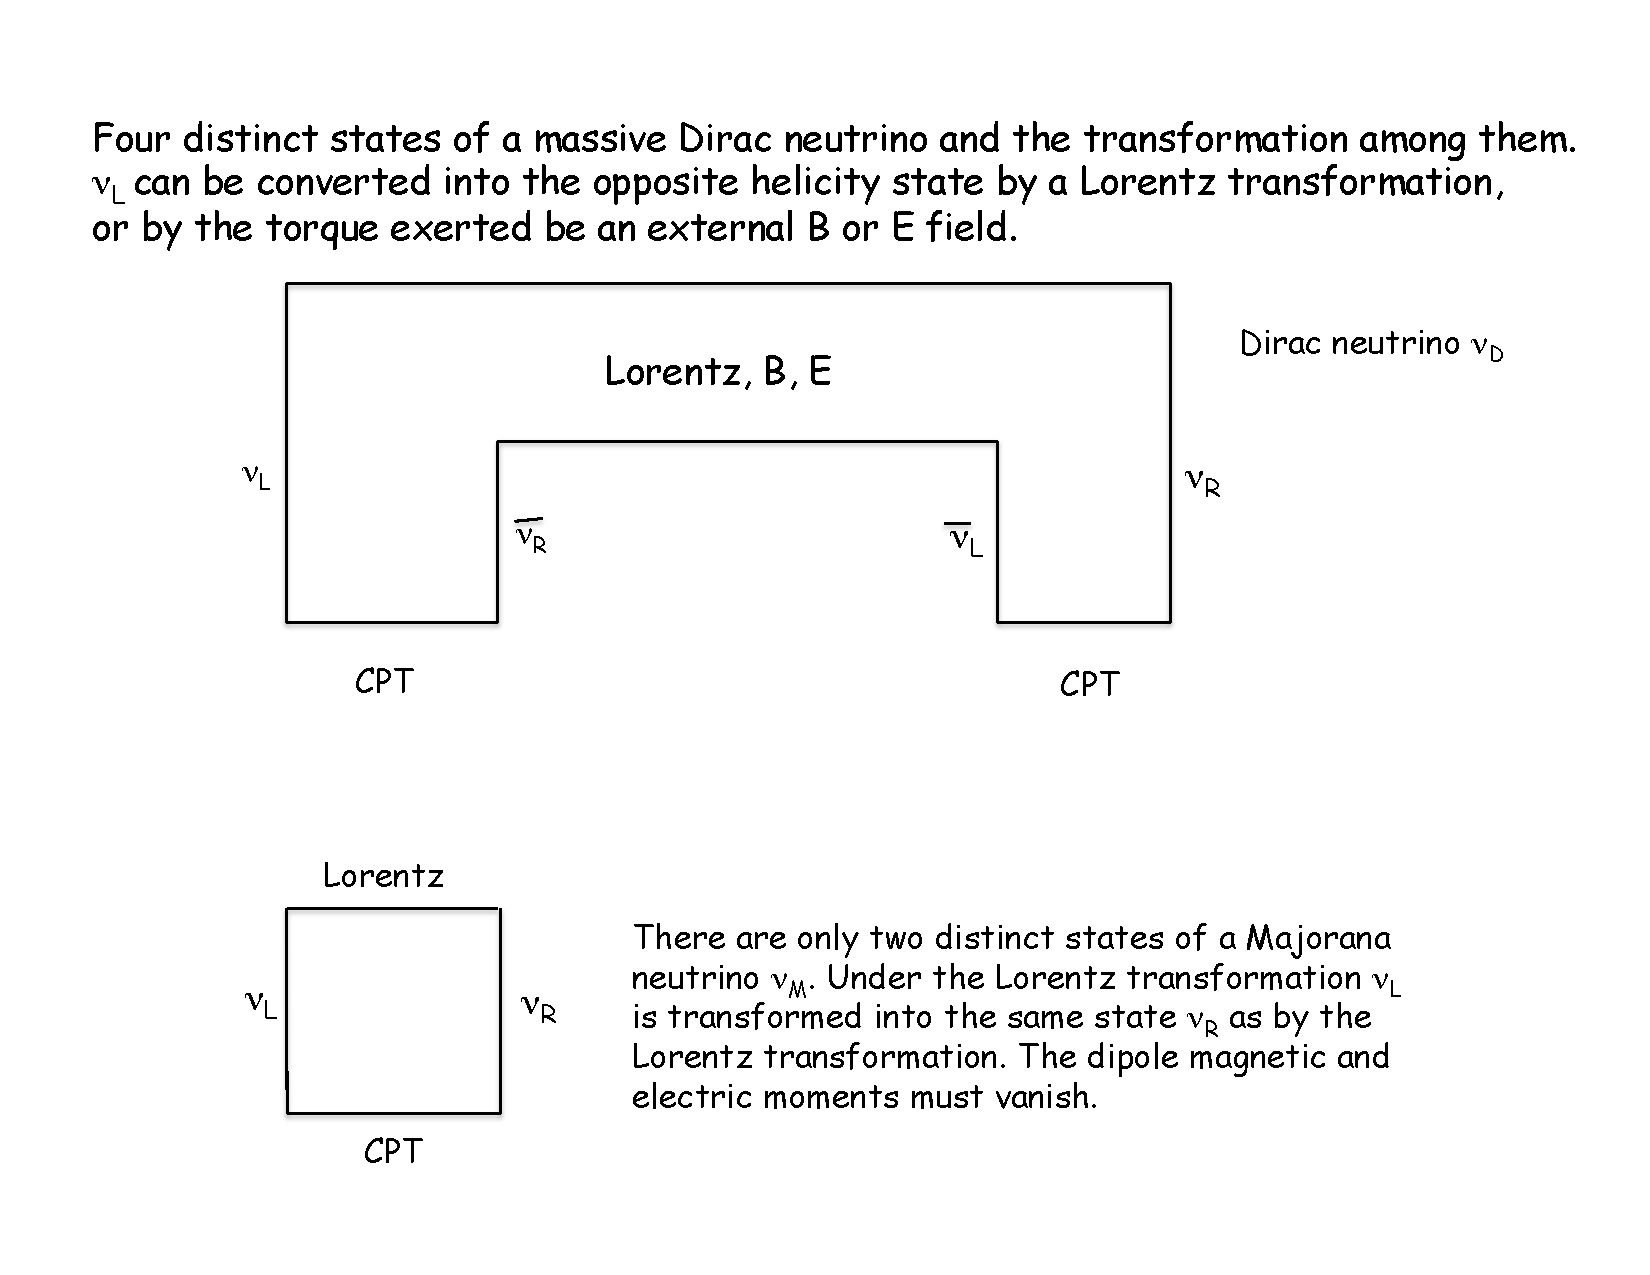
\includegraphics[scale=0.4]{img/DiracVsMajorana2.pdf}
%\end{frame}

\begin{frame}
\frametitle{Dirac or Majorana?}
\begin{columns}
\column{0.45\textwidth}
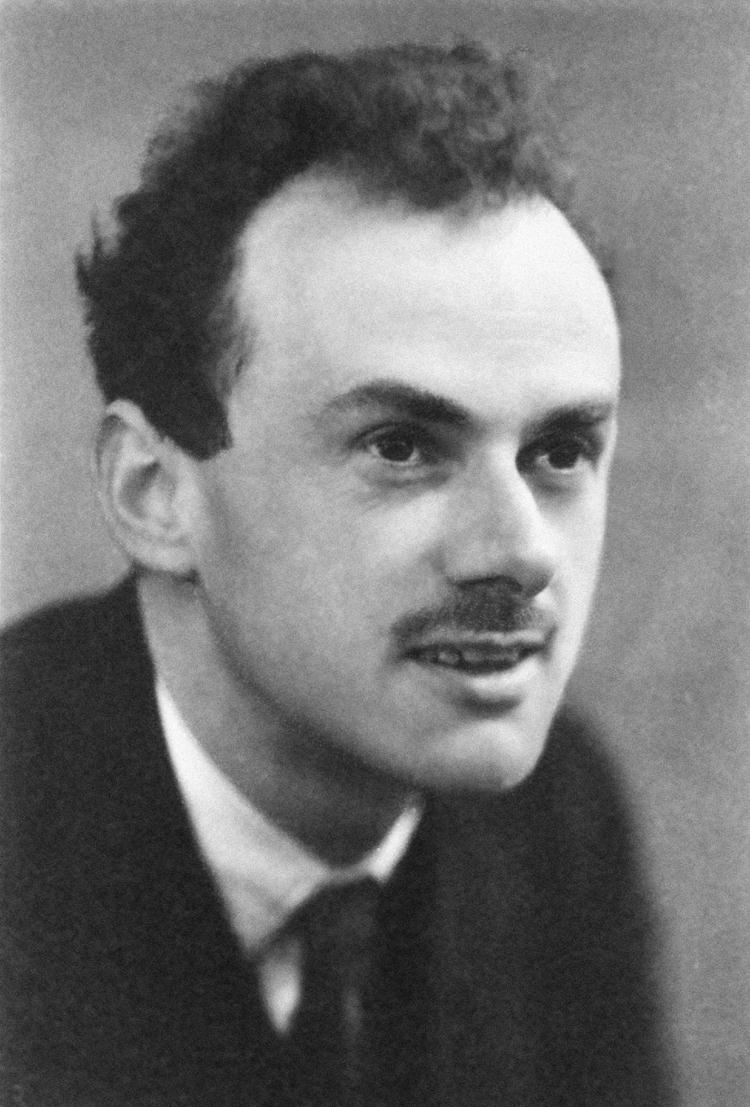
\includegraphics[scale=0.10]{img/dirac_4.jpg}

\begin{empheq}[box=\fbox]{align}
(E +  \va{p}\cdot\va{\sigma}) \chi - m \phi & = &  0 \nonumber \\
(E +  \va{p}\cdot\va{\sigma}) \chi - m \epsilon \chi^* & = & 0 \nonumber
\end{empheq}

\column{0.5\textwidth}
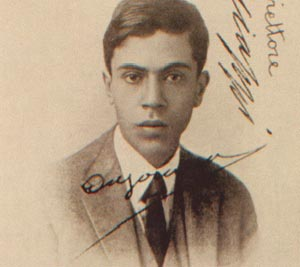
\includegraphics[scale=0.30]{img/Majorana.jpg}

\begin{empheq}[box=\fbox]{align}
(E +  \va{p}\cdot\va{\sigma}) \chi - m \epsilon \chi^* & = 0 \nonumber \\
(E -  \va{p}\cdot\va{\sigma}) \phi - m \epsilon \phi^* & = 0 \nonumber
\end{empheq}

\end{columns}
\end{frame}

\begin{frame}
\frametitle{Deus ex machina}
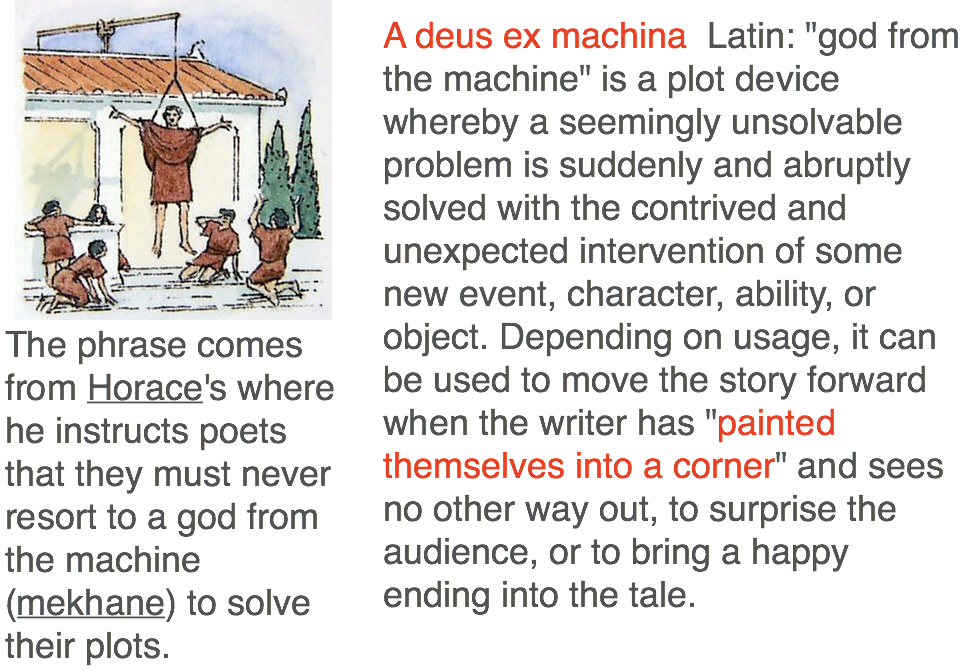
\includegraphics[scale=0.30]{img/DeusExMachina.png}
\end{frame}



%\begin{frame}
%\frametitle{Majorana neutrinos}
%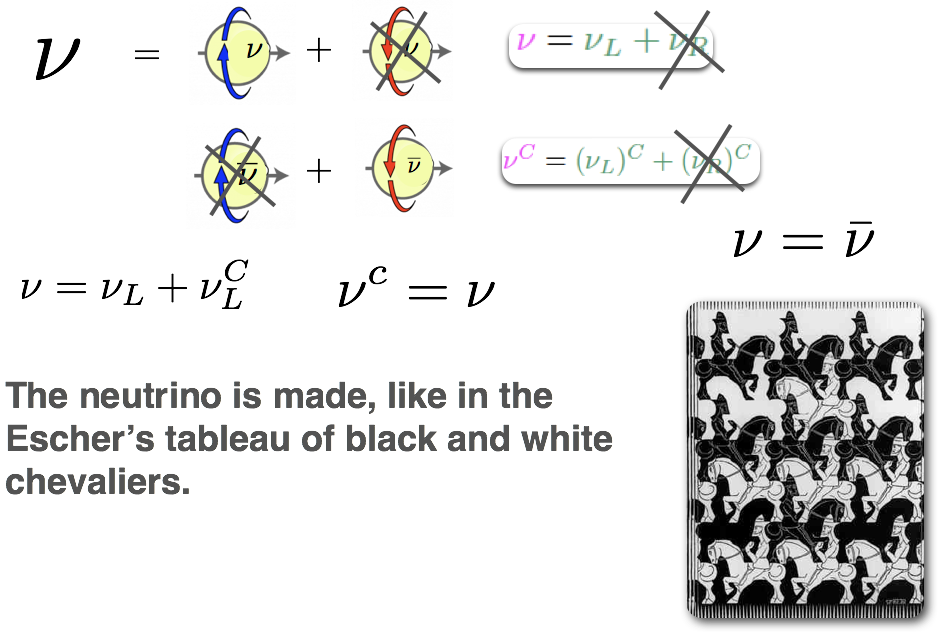
\includegraphics[scale=0.30]{img/MajoranaNeutrinosCartoon.png}
%\end{frame}
%

\begin{frame}
\frametitle{Electron mass in modern QFT: coupling helicity states to the Higgs Field}
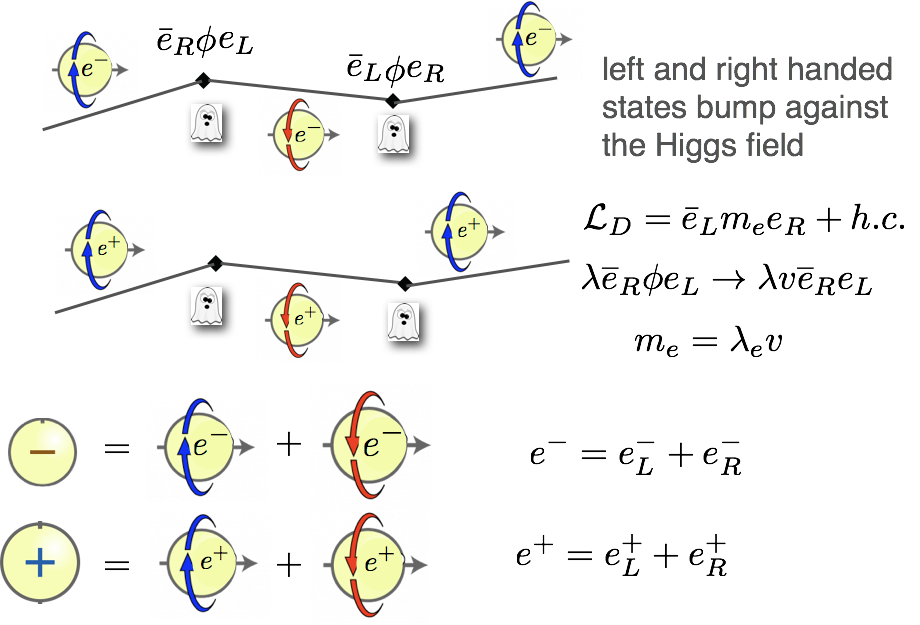
\includegraphics[scale=0.30]{img/ElectronMass.png}
\end{frame}

\begin{frame}
\frametitle{Massive neutrinos can be described by Dirac's equation}
\begin{columns}
\column{0.30\textwidth}
%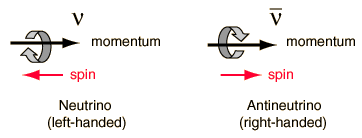
\includegraphics[scale=0.35]{img/NeutrinoHelicity.png}


 \begin{empheq}[box=\fbox]{align}
(E +  \va{p}\cdot\va{\sigma}) \chi - m \phi & = 0 \nonumber \\
(E -  \va{p}\cdot\va{\sigma}) \phi - m \chi & = 0 \nonumber
\end{empheq}


However, unlike the case of the electron, we don't have a "label" (e.g., the electric charge) to separate the unambiguously the particle and the antiparticle. 

\column{0.65\textwidth}
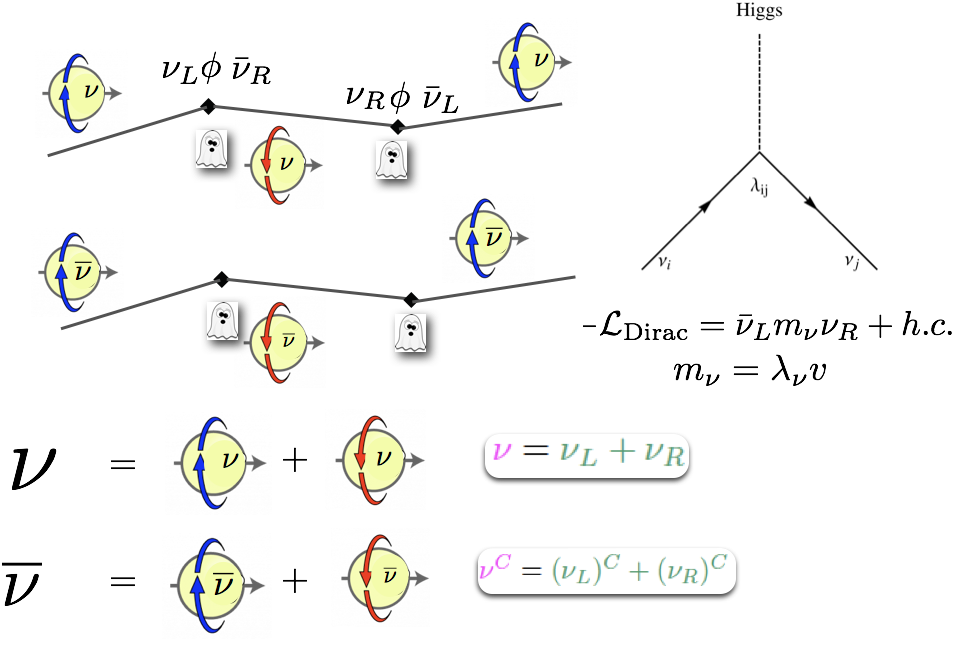
\includegraphics[scale=0.24]{img/NeutrinoMassDirac.png}

\end{columns}
\end{frame}

\begin{frame}
\frametitle{Dirac neutrino mass: Deus ex machina}
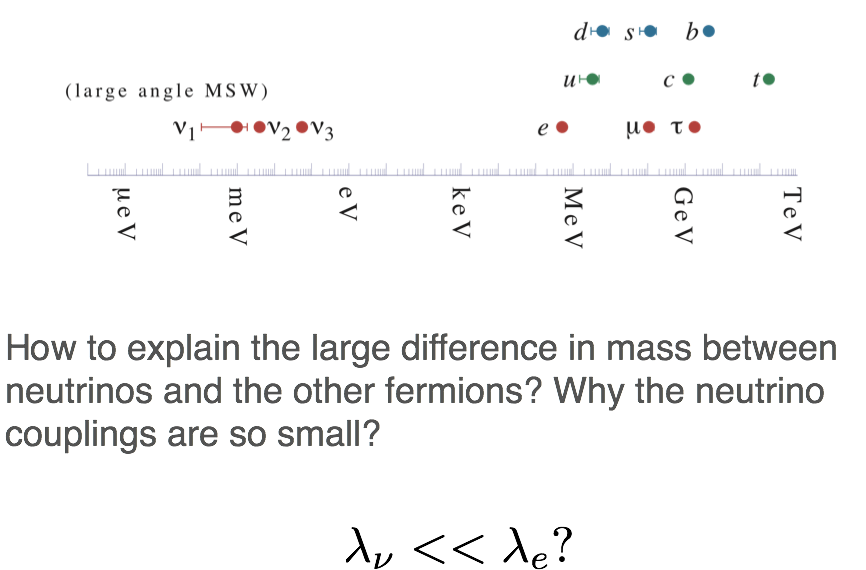
\includegraphics[scale=0.30]{img/SmallNeutrinoMasses.png}
\end{frame}

\begin{frame}
\frametitle{Majorana mass may solve the problem of scale}
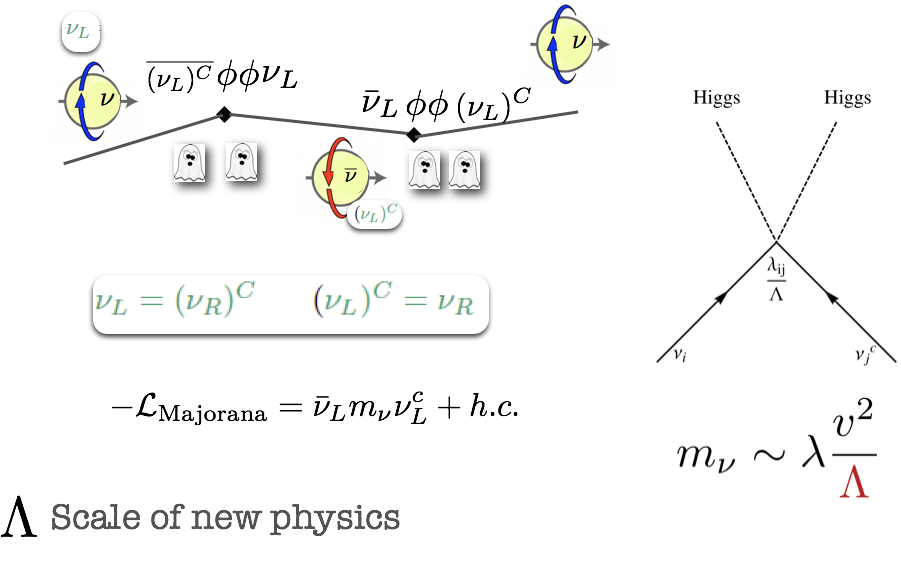
\includegraphics[scale=0.30]{img/MajoranaMass.png}
\end{frame}

%\begin{frame}
%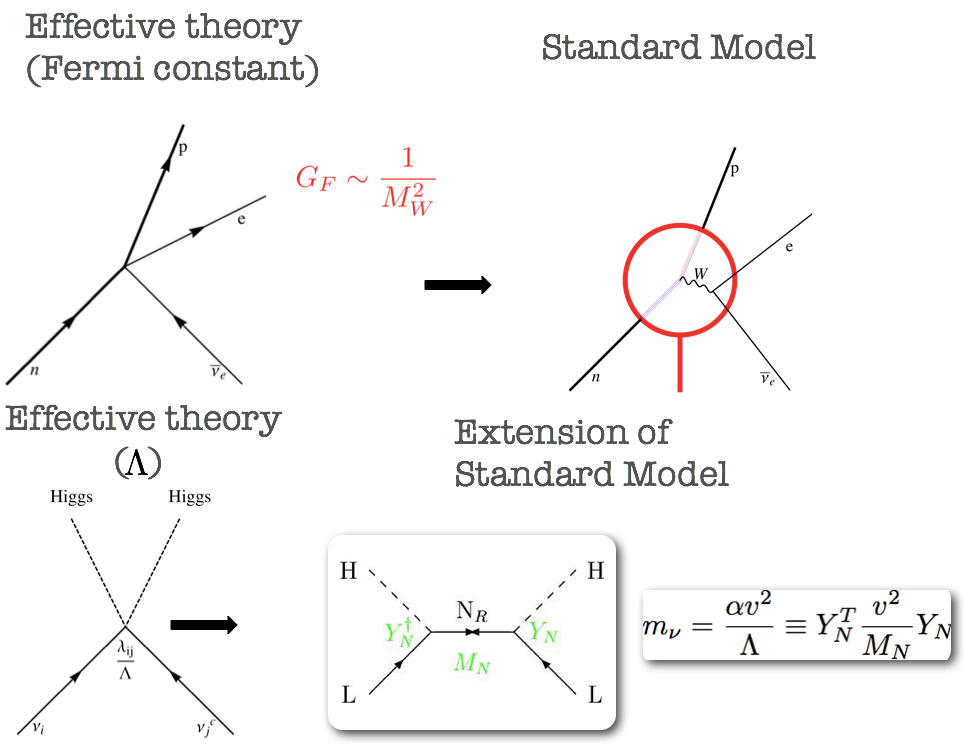
\includegraphics[scale=0.30]{img/Effective.png}
%\end{frame}



\begin{frame}
\frametitle{The mystery of the missing antimatter}
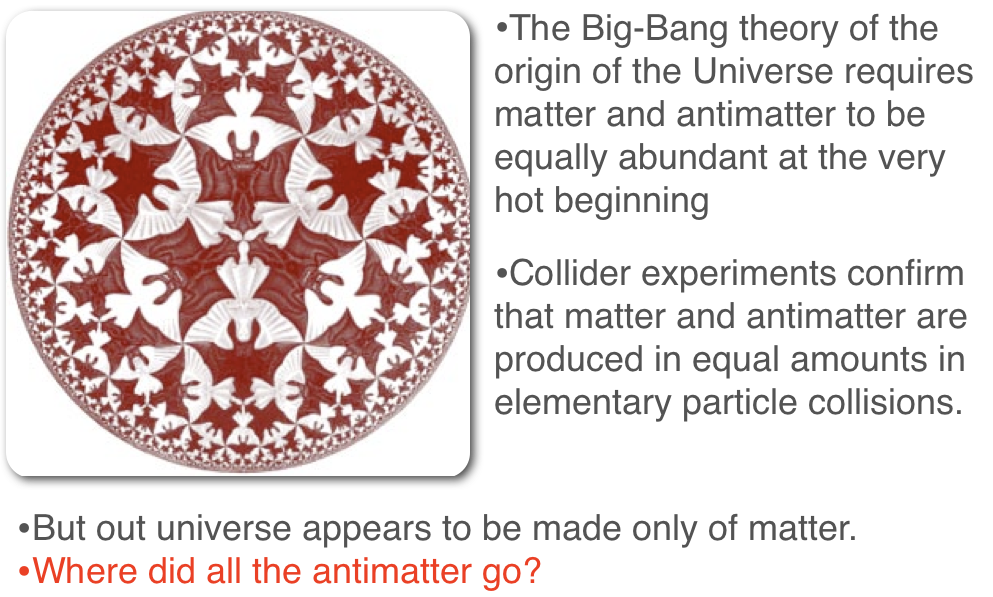
\includegraphics[scale=0.30]{img/MissingAntiMatter.png}
\end{frame}

\begin{frame}
\frametitle{CP violation and Majorana neutrinos}
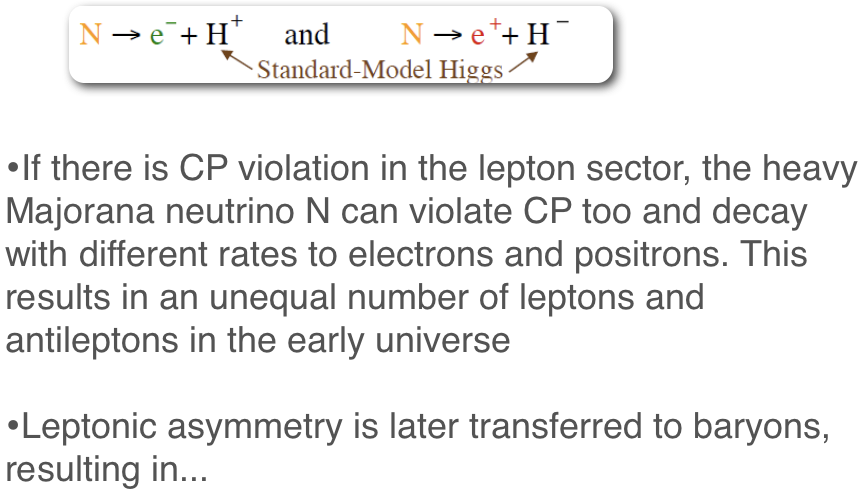
\includegraphics[scale=0.30]{img/CP.png}
\end{frame}

\begin{frame}
\frametitle{We are the leftovers}
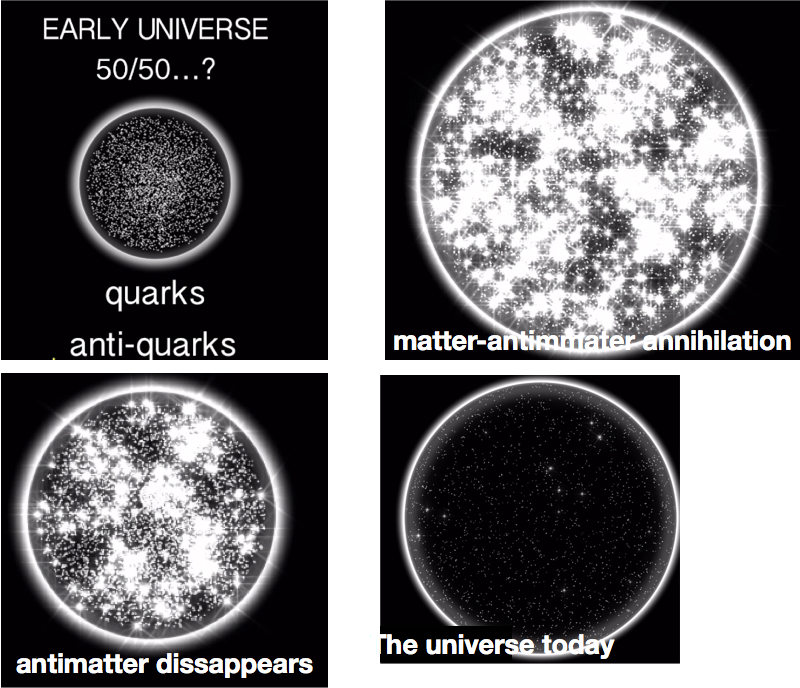
\includegraphics[scale=0.30]{img/MissingUniverse.png}
\end{frame}
%

\begin{frame}
\frametitle{A formula for the Universe}
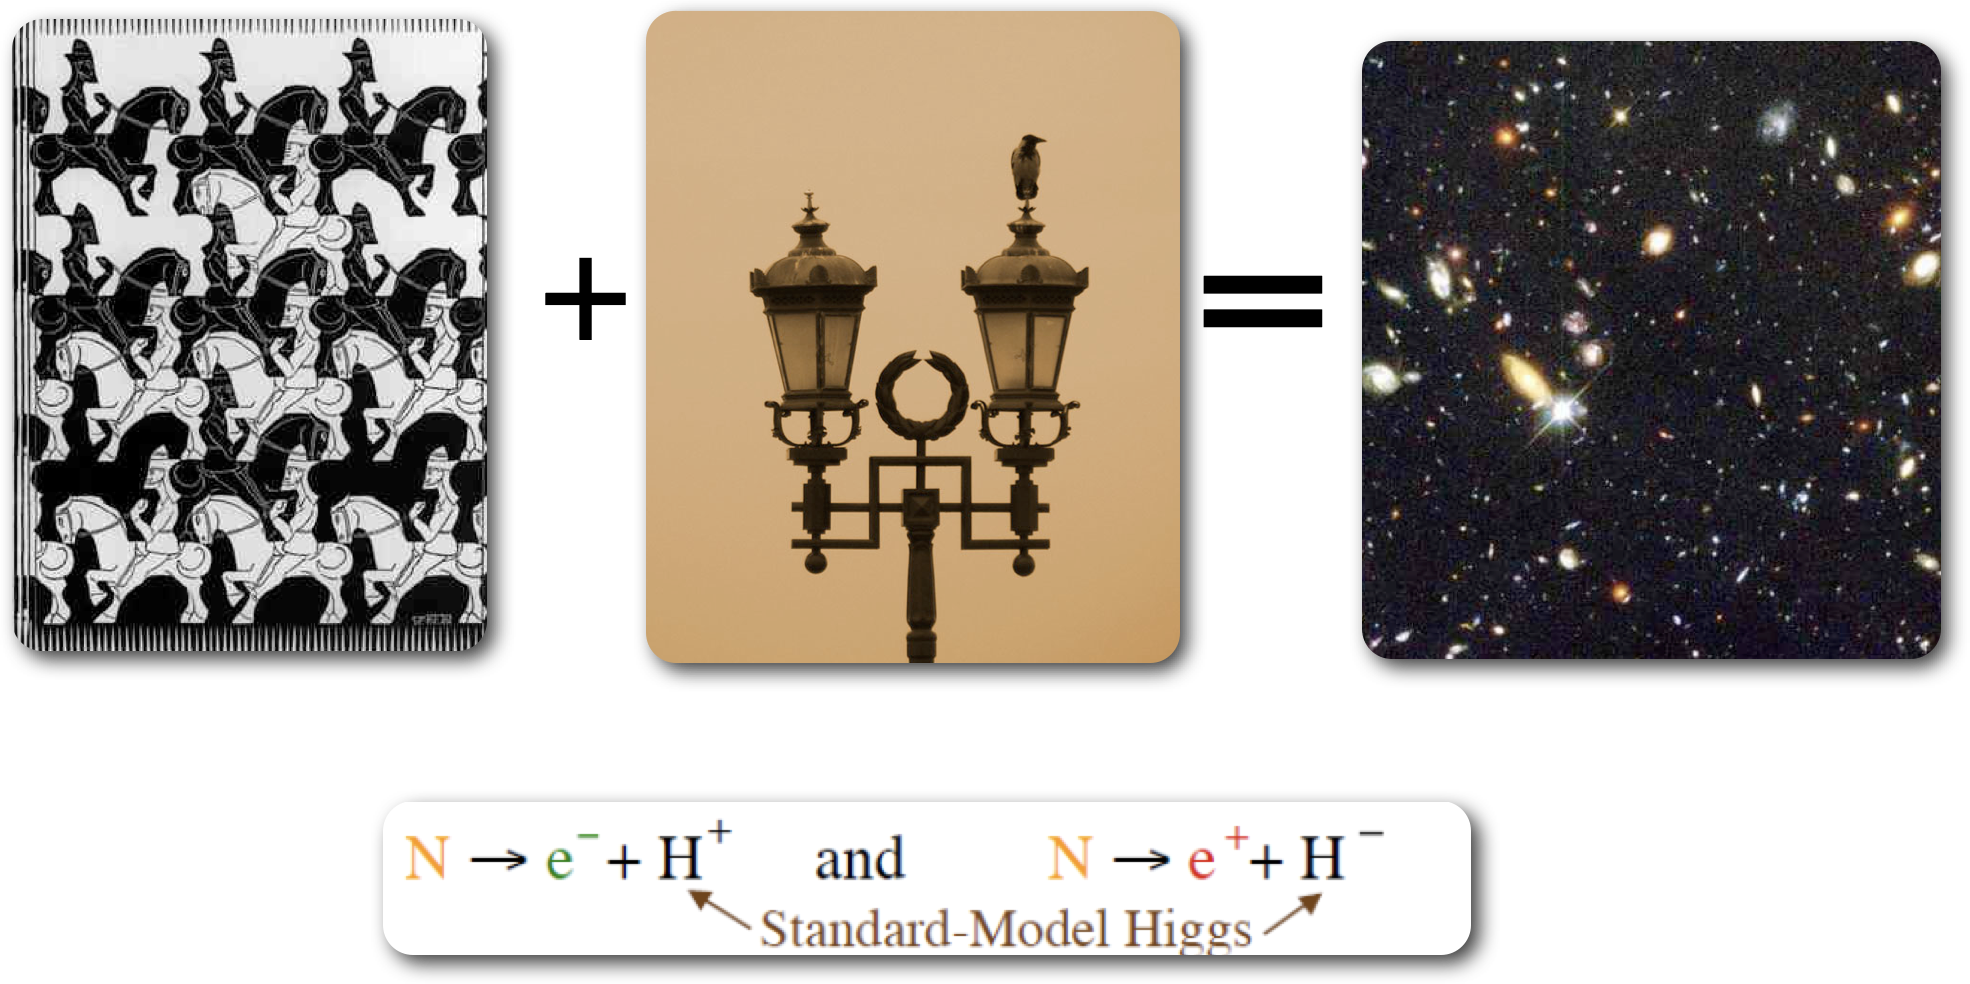
\includegraphics[scale=0.30]{img/formulaUniverse.png}
\end{frame}


